\chapter{Kommuneplan}
En kommuneplan er kommunens overordnede plan for kommunens udvikling. Indenfor en periode på 12 år fastlægger kommunen de overordnede mål og retningslinjer for kommunens udvikling såvel i byerne som i det åbne land. 
\newline
\newline
En kommuneplan består af; en hovedstruktur, retningslinjer, kommuneplanrammer, bilag og tilhørende planredegørelse. 
\newline \indent{     }  Hovedstrukturen er den overordnede, strategiske og sammenfattende fysiske plan for kommunen. Den fastlægger de overordnede mål for udviklingen inden for de enkelte sektorer for hele kommunen og for de enkelte områder. 
\newline \indent{     }  Retningslinjerne udgør de overordnede rammer for kommuneplanlægningen. De fastsætter principperne for arealanvendelsen i kommunen, og danner ligeledes grundlag for kommunens administration af planlovens landzonebestemmelser, samt administrationen af kompetencer indenfor anden lovgivning, herunder natur-, miljø-, bygge- og vejlovgivningen og husdyrloven. Retningslinjerne angiver sammen med områdeudpegningerne hvilke forhold, der skal tages hensyn til i administrationen, og hvilke konkrete skøn der skal foretages for disse områder. 
\newline \indent{     }  Kommuneplanrammerne styrer den overordnede arealanvendelse og danner ramme for indholdet i nye lokalplaner. Planrammerne fastlægger dermed mål, muligheder og begrænsninger for arealanvendelse i de enkelte dele af kommunen. Kommuneplanrammerne har to niveauer: 1) by/bydel/landområde og 2) rammeområder. Det første niveau “by/bydel/landområde”, behandler områdets særlige problemer, værdier og muligheder i en sammenhæng. Det andet niveau “rammeområder”, er det mest detaljerede niveau i kommuneplanen rent geografisk. Her fastsættes de bestemmelser der danner grundlag for lokalplaner.
\newline \indent{     }  Bilag er de generelle rammebestemmelser, hvor der henvises til de aktuelle bilag fra de enkelte emner.
\newline \indent{     }  Planredegørelser beskriver forudsætninger for, og ændringerne i den konkrete planlægning. Byrådet offentliggør, sammen med alle kommuneplanforslag eller med forslag til kommuneplantillæg\footnote{Opstår der problemer med at realisere en lokalplan ud fra kommuneplanen, så anvendes der et kommuneplantillæg, som er et supplement til den eksisterende kommuneplan. Denne kan justere og ændre bestemmelserne i kommuneplanen, for at gøre det muligt at realisere lokalplanen \citep{kommuneplan2009}.}, en redegørelse om planens baggrund og sammenhæng med anden planlægning. Kommuneplanen ledsages også af en planredegørelse og planstrategi, hvilken laves minimum hvert 4. år i tilknytning til kommunens budget. Denne er byrådets instrument og baner vejen for at realisere kommuneplanens mål. Her oplyses blandt andet om kommuneplanens væsentlige forudsætninger, planlægninger der er gennemført det forgangne år, det kommende års kommuneplaninitiativer samt byrådets vurdering af og strategi for udviklingen for både det kommende år (budgetåret), de kommende 4 år (overslagsårene) og en længere periode på 12 år. Desuden laves der jævnligt statusredegørelser, som giver et overordnet billede af kommunens fysiske udvikling og præsenterer de økonomiske tiltag, der knytter sig til kommunens sektorer og geografiske områder \citep{kommuneplan1}.

\section{Aalborg Kommuneplan}
Aalborg Kommuneplan beskriver kommunens udvikling inden for de 12 kommende år og er opdelt i fem fokuspunkter: 
\begin{enumerate}
\item Byerne - et godt sted at bo hele livet
\item Nødvendige forbindelser - mobilitet
\item Det åbne land
\item Bæredygtighedsprofil
\item Aalborg - den attraktive storby
\end{enumerate}
Et af Aalborg Kommuneplans fem fokuspunkter er “Byerne - et godt sted at bo hele livet”. De større byer under Aalborg Kommune har, i kraft af nærheden til Aalborg, en god infrastruktur,  et varieret serviceudbud samt tilstrækkeligt befolkningsunderlag. Det er et særligt potentiale for byvækst, der skal udnyttes for at understøtte Aalborg som Norddanmarks Vækstdynamo. 
\newline \indent{     }  Byvæksten skal have særligt fokus på nye, kreative boligformer, som tilgodeser klimaudfordringer, demografiske udfordringer og bæredygtighed. 
\newline \indent{     }  Ikke kun de større byer nær Aalborg har en væsentlig rolle i projektet. Mindre byer og landsbyer er også i fokus, og har en særlig rolle som opland til Aalborg med store kvaliteter indenfor bosætning, rekreation og friluftsliv.
\newline
\newline
Et andet af Aalborg Kommuneplans fem fokuspunkter er “Nødvendige forbindelser - mobilitet”. Dette fokuspunkt omhandler byens behov for forbindelser, der kan håndtere transportbehovet og gøre det mere attraktivt at benytte offentlig transport såsom bus og tog, samt at tage cyklen, da  Aalborg Kommune har en målsætning om at blive Danmarks førende cykelby. Kommunens mål er færre bilkøer, god adgang til indkøb, service og arbejdspladser samt sikring af forbindelser, der understøtter en effektiv godstransport. Derudover satser Aalborg på en letbane som det bærende element i byen.
\newline
\newline
Fokuspunktet “Det åbne land” omhandler benyttelsen og beskyttelsen af det åbne land. Dette skal ske på et bæredygtigt grundlag med plads til oplevelser, natur, erhvervsinteresser og vedvarende energi. Det åbne land skal danne ramme om levende og aktive områder.
\newline
\newline
Aalborg Kommune har også stor fokus på bæredygtighed og har dertil punktet “Bæredygtighedsprofil”. Udviklingen af et bæredygtigt samfund omhandler flere punkter, såsom at passe på miljøet, klimaet og naturen, om at bygge byer for mennesker og om at få det bedste ud af den nuværende økonomiske virkelighed. En bred tilgang til bæredygtighed er derfor udgangspunktet \citep{kommuneplan2}.

\subsection{Aalborg Vækstakse}
Det femte og sidste fokuspunkt i Aalborgs kommuneplan er “Aalborg - den attraktive storby”. Dette fokuspunkt indeholder yderligere tre punkter; vækstaksen som byens motor, byudviklingsprincipper for Aalborg og fokus på bykvalitet. 
\newline
\newline
Aalborg Kommune har valgt at koncentrere sig om et vækstbånd, kaldet Vækstaksen, som skal danne grundlag for Aalborgs udvikling, hvor der er fokus på det generelle udviklingsprincip. Området går fra Aalborg Lufthavn i vest, gennem midtbyen, til Campus og videre ud til østhavnen, hvilket illustreres på Figur \ref{fig:vaekstakse}. 
\newline \indent{     }  Blandt Vækstaksens mest centrale elementer er færdiggørelsen og videreudviklingen af en række større områder i Aalborg, som for fremtidig skal være med til at skabe Aalborg som storby og præge dens identitet. Gennem disse færdiggørelser vil bykvaliteten øges, og byen vil blive mere attraktiv. Der lægges derfor stor vægt på arkitektoniske overvejelser samt historiske skulpturer og monumenter, når der skal bygges og renoveres. 
\newline \indent{     }  Her har havnefronten, som et af de første områder, gennemgået en stor renovering, hvor der er etableret både Havenebad, Jomfru Ane Parken og sportsfaciliteter. Derudover blev Tivoli Karolinelund fjernet i 2011, og i 2012 åbnede en ny Karolinelund park, som nu danner ramme for mange forskellige nichekulturer, såsom koncerter, Platform 4, legepladser og meget mere, og parken er fortsat under udvikling \citep{jomfruaneparken} \citep{karolinelund}. 
\newline \indent{     }  Aalborg er gennem renoveringen af den nye havnefront også vokset som kulturby, og i dag er kultur blevet en bærende del af byen, hvor der findes KUNSTEN museum, Aalborg Kultur og Kongres center, Nordkraft samt det nye Musikkens Hus, der åbnede i 2014, hvor der hver uge afholdes forskellige koncerter og andre arrangementer. Dette er altsammen med til at styrke Aalborg som vækstby og byens erhvervsturisme. Ligeledes er der planer om en ny kulturbro på Jernbanebroen, som også skal være med til at styrke kulturen i Aalborg og Aalborg Kommune. Ved at styrke kulturen styrkes bykvaliteten også, og byen bliver en levende by, hvor det er muligt at binde shopping, café og kulturliv sammen \citep{kulturbro} \citep{musikkenshus}.
\newline \indent{     }  Den gamle Eternitgrund i Aalborg havde i en lang årrække stået ubrugt hen, men gennem de sidste fem år er der etableret både studieboliger, supermarkeder, fitnesscenter og et nyt legeland for børn. Virksomheder som Plus Bolig og COWI er ligeledes flyttet ned på Eternitten, og i dag er Eternitten blevet en stor drivkraft for Aalborg,  hvor der fortsat  er fremtidige planer om grønne arealer også \citep{eternitten}.
\newline \indent{     }  Projektet om Vækstaksen er i fuld gang, og inden for den nærmeste fremtid skal også Godsbanearealet og det østlige Aalborg udvikles, for at øge oplevelsesmulighederne, kulturtilbudene og skabe attraktive og bæredygtige livsvilkår her. Det er dog ikke kun nybyggerier, som Vækstaksen har fokus på. For Aalborg Kommune er det også vigtigt, at vedligeholde de gamle bygninger, for at opretholde byens historisk identitet.

\begin{figure}[htbp]
	\centering
	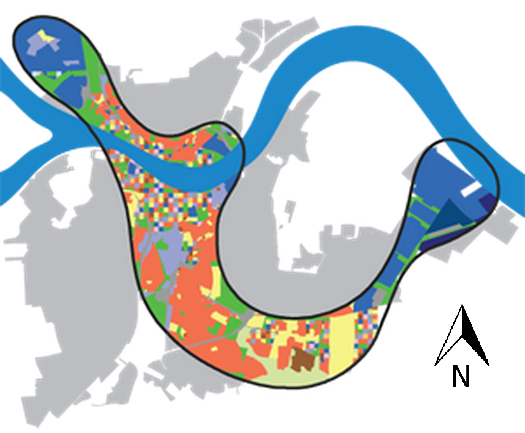
\includegraphics[width=0.5\textwidth]{billeder/vaekstaksen.png}
	\caption{Aalborgs Væsktakse}
	\label{fig:vaekstakse}
\end{figure}

Vækstaksen skal være attraktivt for alle aldersgrupper og skal derfor have noget, at tilbyde hver enkelte borger, og skal ligeledes være med til at skabe oplevelsesmuligheder og kulturtilbud.
\newline \indent{     }  En stor del af planerne for Vækstaksen er byfortætning, mobilitet, studieby og miljø. 
Der er i Aalborg Kommune stor udviklingspotentiale inden for byfortætning. På Figur \ref{fig:udvikling} ses udviklingspotentialet i Vækstaksen. De markerede lilla områder er der hvor Aalborg Kommune har bedst udviklingspotentiale.
\newline \indent{     }  Dette udviklingspotentiale er i form af tilbyggelse og omdannelse af boliger, arbejdspladser og naturområder. Byfortætning kan resultere i en meget presset infrastruktur, derfor er mobilitet et essentielt punkt for optimering af byens potentiale. Det er vigtigt, at der er let og hurtigt adgang til offentlig transport, og det skal gøres mere attraktivt, at tage cyklen. Målet er, at få en stor by til at opfattes som en “lille by”, ved at gøre transport lettilgængeligt og derfor nemt at komme fra bydel til bydel. Infrastrukturen vil styrkes blandt andet via en cykelmotorvej samt en kommende letbane, som skal forbinde Østhavnen, Campus, det kommende superhospital i Aalborg Øst, midtbyen og ud til Aalborg Lufthavn.

\begin{figure}[htbp]
	\centering
	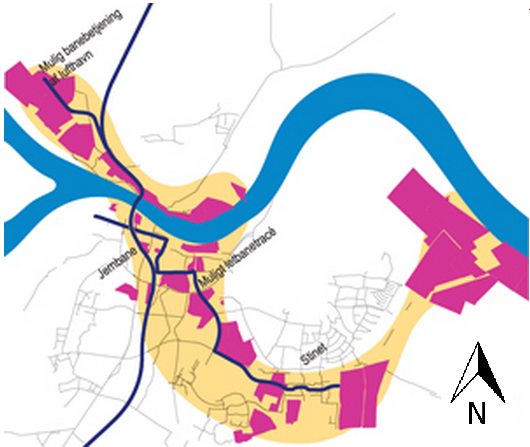
\includegraphics[width=0.5\textwidth]{billeder/udvikling.png}
	\caption{Udviklingspotentiale}
	\label{fig:udvikling}
\end{figure}

Ved Vækstaksens to endepunkter ligger Aalborgs største industriområder, Aalborg Østhavn og Aalborg Lufthavn. Disse industriområder er kommet til efter industrifirmaer er begyndt at flytte fra havnefronten og ud til yderkanten af Vækstaksen. Trods denne flytning forbliver Aalborg en erhvervsby samtidig med, at den gradvist omdannes til en studieby. De store industrifirmaer er stadig vigtige for Aalborg, da de er med til at skabe omsætning og arbejdspladser. 
\newline \indent{     }  Da Aalborg gradvist omdannes til en studieby, er det vigtigt, at der i Vækstaksen støttes op om Aalborgs studieliv og studiemiljø, da 10\% af Aalborg Kommunes befolkning består af studerende \citep{campus}. Et godt studiemiljø vil styrke innovation, konkurrence og vækst i erhvervslivet. Det er nødvendigt med gode uddannelsesmuligheder, faciliteter samt ungdomsboliger til de studerende, hvilket også vil gøre det attraktivt for udefrakommende at studere i Aalborg. Centrum for studielivet i Aalborg udspringer fra Campus i Aalborg Øst, hvor størstedelen af de videregående uddannelser findes. 
\newline
\newline
Aalborg Kommune ønsker også at udvikle byens natur og udendørsliv. Til at opnå dette vil kommunen opføre parker, stisystemer og vandløb. Vandløbene vil give byen historisk identitet, samtidig med at de vil beskytte byen under eventuel øget vandstand, da de kan forsinke vandet. Formålet med parkerne og et naturrigt Aalborg er at skabe et sundhedsfremmende forhold for alle aldersgrupper og beskytte klimaet. Desuden vil Aalborg Kommune gøre Aalborg til en miljøvenlig storby, hvilket vil gøre byen til en attraktiv by, og dermed øge indbyggertallet. Derfor vil Aalborg Kommune genoprette naturen og give velfærd til byens borgere \citep{kommuneplan3}.

\section{Lokalplan}
En lokalplan tager udgangspunkt fra en fremsat kommuneplan og har til formål at styre udviklingen i et område. Lokalplanen skal give borgerne og byrådet et indblik i et bestemt område og give dem mulighed for at komme med tiltag til den fremlagte plan. Her fastsætter byrådet rammerne for, hvordan arealer, bygninger, beplantning, veje, stier mv. skal anlægges i et givent område. Lokalplaner skal ifølge planloven udformes af byrådet, der har pligt til dette, før der kan gennemføres større bygge- og anlægsprojekter.
\newline
\newline
En lokalplan indeholder punkterne; redegørelse, planbestemmelser og bilag.
\newline \indent{     }  Planen starter med en redegørelse, hvor lokalplanens baggrund og formål fastsættes og hele indholdet fremlægges. Der bliver også redegjort for miljømæssige forhold, hvordan lokalplanen forholder sig til andet byggeri, og om der kræves tilladelser eller anden slags dispensationer fra forskellige myndigheder.  
\newline \indent{     }   I lokalplanen informeres der om planbestemmelser, som er områdets fremtidige anvendelse. Dette illustreres via tekst og billeder.
\newline \indent{     }  Til sidst i lokalplanen ligger alle bilagene. Disse består oftest af forskellige kort (matrikelkort, arealanvendelseskort m.m) samt forskellige tabeller omkring støj fra erhverv og trafik m.m. Bilagene er med til at uddybe og illustrere lokalplanbestemmelserne.
\newline
\newline
Byrådet kan til enhver tid udarbejde et lokalplanforslag. Når et forslag til lokalplanen er udformet, skal det offentliggøres i mindst 8 uger, hvor borgerne kan komme med indsigelser eller forslag til ændringer. Efter de 8 ugers offentliggørelse bedømmer byrådet, hvorvidt eventuelle indsigelser eller ændringer vil blive taget op. Dernæst vedtages planen, hvor den bekendtgøres i avisen og er hermed bindende for ejendommene, som ligger i lokalplanområdet.
\newline \indent{     }  Der må ikke laves ændringer i området i strid med lokalplanen, dog må eksisterende bebyggelser og anvendelse, der er etableret før lokalplanforslagets offentliggørelse, fortsætte. Endvidere er der ikke pligt til at gennemføre tiltag, der beskriver lokalplanen (\citep{lokalplan}, s. 4).

\subsection{Lokalplan 1-1-107}
Lokalplan 1-1-107 er lokalplanen for området ved Strøybergs Palæ. Den er udarbejdet i forbindelse med et ønske om, at lave en tilbygning til Strøybergs Palæ, hvor anvendelsesmulighederne i området således vil blive ændret til både beboelse, serviceerhverv og kontorerhverv, frem for kun erhverv, som Strøybergs Palæ primært bliver anvendt til i dag. Lokalplanen er udformet således, at den tager hensyn til at den nye bebyggelse udformes efter den eksisterende bevaringsværdige bygning, eventuelt med et nutidigt arkitektonisk udtryk, således der er harmoni mellem den nuværende bygning og tilbygningen. Her tages der hensyn til bygningsskala, facaderytme og farve, da Strøybergs Palæ er vurderet til at være en bevaringsværdig bygning med en bevaringsværdi 4 (middel) (\citep{lokalplan}, s. 5 og 9). Desuden skal tage udføres som sadeltage eller som flade tage (\citep{lokalplan}, s. 17).
\newline
\newline
Området for lokalplanen er ca. 1200 $m^2$, og ligger ca. 100 m fra Limfjorden. Øst for lokalplanområdet ligger Gammel havn, mod nord og vest ligger Utzonparken og mod syd Nyhavnsgade. Ud over Strøybergs Palæ, der ligger i planområdet, er der også enkelte mindre bygninger, garager mm. For at lokalplanen kan blive realiseret, skal mindre bygninger nedrives, hvis de ikke er bevaringsværdige (\citep{lokalplan}, s. 6).
\newline \indent{     }  Da lokalplanområdet ligger meget kystnært skal der i større grad dimensioneres efter klimatiske faktorer og ændringer. Her er hovedpunktet vandstandsstigning. Her tages der udgangspunkt fra Aalborg Kommunes klimastrategi. Den forudsiger at den generelle indre vandstand i nordjyske farvande vil kunne stige med op til en meter. Derfor er der fastsat en minimum sokkelkote for stueplan på nye bygninger på 2,36 m. DVR 90 på grund af risikoen for vandstandsstigning (\citep{lokalplan}, s. 9).
\newline \indent{     }  Bygningen ligger placeret tæt opad detailhandel og erhverv. Området betjenes af kollektiv trafik. Da bygningen ligger placeret ved Nyhavnsgade, kan dette give støjgener fra trafikken. Derfor skal der tages højde for dette, når der bygges. Det indendørs støjniveau må ikke overstige $L_{den}$ 33 dB, samt ved udendørs opholdsarealer må denne ikke overstige $L_{den}$ 58 dB. Støjisolering skal primært ske indvendigt, så bygningen ikke ændrer udseende. Overholdelse af de forskellige grænseværdier for støj skal kunne dokumenteres, før bygningen må tages i brug (\citep{lokalplan}, s. 8).
\newline
\newline
Lokalplanen indeholder to delområder, hvor delområdet A er hovedbygningen af Strøybergs Palæ, mens delområde B er sidebygningen dertil og et byggefelt liggende mod nord. Alt ny bebyggelse her skal etableres i 3 etager plus en tagetage. Herudover kan der laves en høj kælder, som kan anvendes til parkering, depot eller lignende. Kælderen må højest have en lofthøjde på 2 m over terræn og tilbygningen må højest være 19 m høj (\citep{loaklplan}, s. 7).
\newline \indent{     }  Lokalplanen skal udarbejdes i sammenspil med den nuværende kommuneplan og anden fysisk planlægning i området omkring. Derfor laves der også tillæg til kommuneplanen, så denne stemmer overens med lokalplanen. Lokalplanens dækkende område er skrevet ovenover, og planen er, at der i dette område kan indrettes et mindre antal boliger. Det forventes at Aalborg midtby får etableret 2116 nye boliger i perioden 2008-2019. I bygningen kan desuden etableres butikker på maks 250 $m^2$  og 500 $m^2$ pr. etage jf. kommuneplanen (\citep{lokalplan}, s. 8).